%*******************************************************************
% Chapter 5: Proposed Methodology
%*******************************************************************

\section{Design Process Overview}

The proposed methodology follows four phases: (1) multimodal dataset curation from heterogeneous public sources, (2) design and comparison of six fusion architectures, (3) training with missing-modality simulation (synthetic corruptions are applied only in separate offline stress tests), and (4) evaluation on a held-out test set. Figure~\ref{fig:pipeline_overview} shows the end-to-end pipeline from raw sensor inputs to classification output.

\begin{figure}[H]
\centering
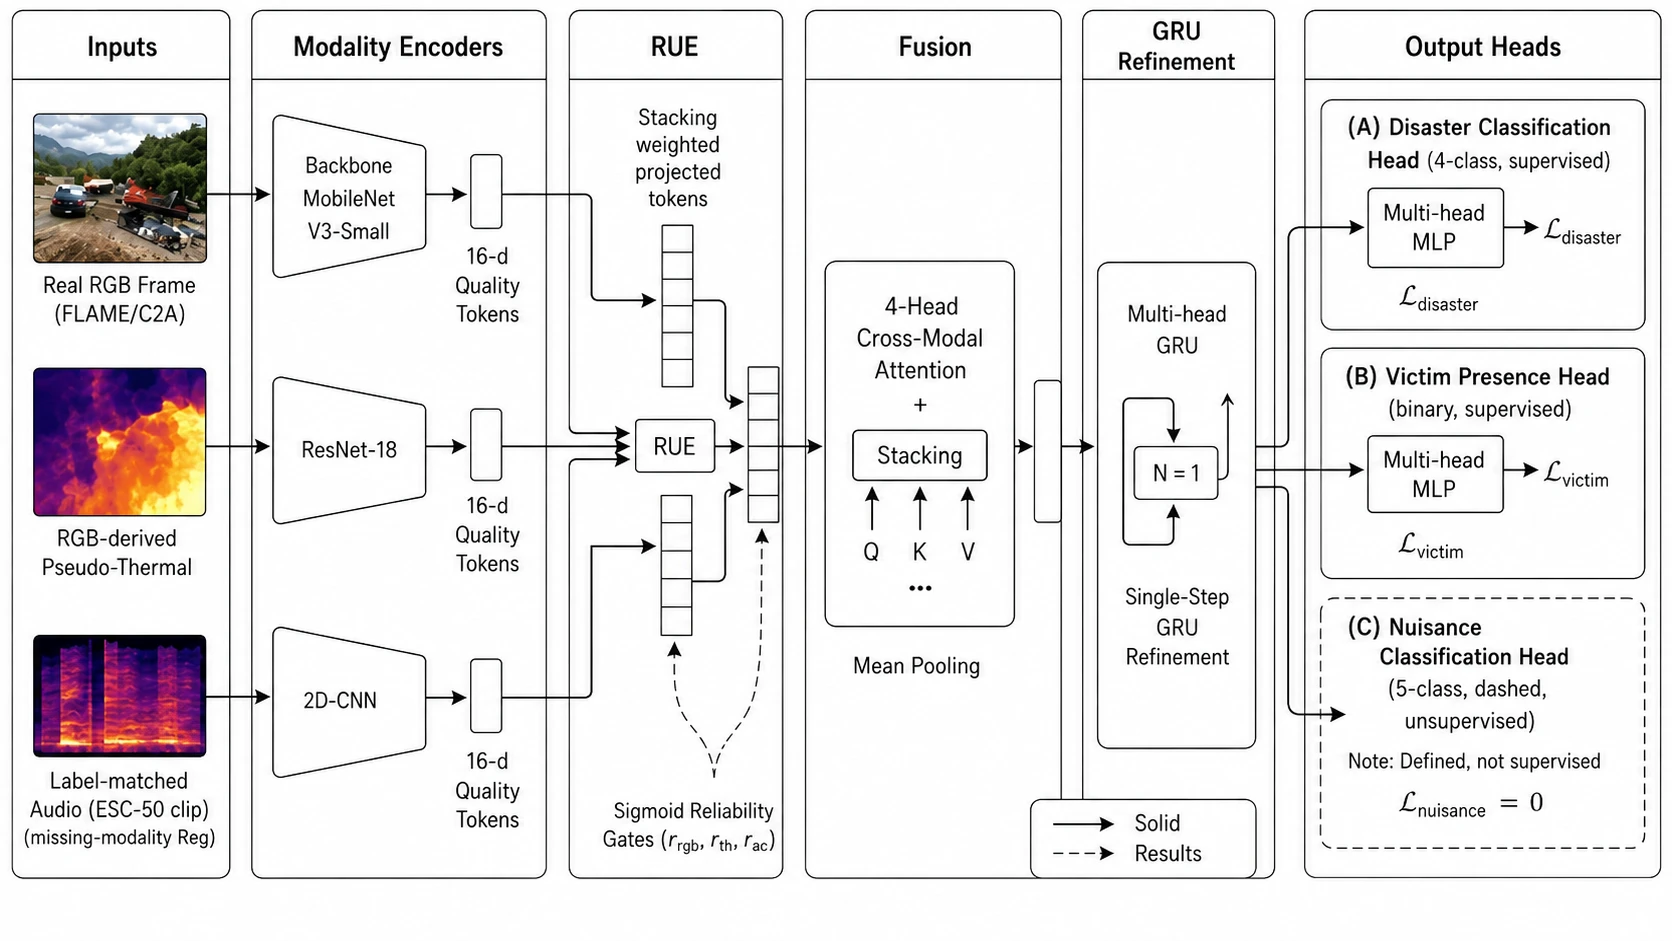
\includegraphics[width=\textwidth]{images/generated/4.1.png}
\caption{Evidence-grounded AdapFuse-v1 computational graph. RGB, RGB-derived pseudo-thermal, and optional label-matched audio are encoded and projected to three 192-d tokens. RUE gates modulate the tokens before four-head attention and mean pooling. The GRU is executed with sequence length one in the current loader and therefore acts as a gated refinement block, not temporal memory. Disaster and victim-presence heads are supervised; the dashed nuisance head is defined but receives no nuisance labels in our trainer.}
\label{fig:pipeline_overview}
\end{figure}

\section{Dataset Curation}

\subsection{Sources and Composition}
\label{sec:dataset_sources}

Because no single public dataset provides synchronized RGB, thermal, and audio for UAV disaster detection, the dataset was assembled from six public sources and unified under a structured metadata catalogue. Table~\ref{tab:dataset_sources} lists each source, the disaster scenario it covers, and its contribution.

\begin{table}[H]
\centering
\caption{Dataset Sources and Contribution to the Unified Metadata}
\label{tab:dataset_sources}
\resizebox{\textwidth}{!}{%
\begin{tabular}{@{}llccp{5cm}@{}}
\toprule
\textbf{Source} & \textbf{Scenario} & \textbf{Modalities} & \textbf{Samples} & \textbf{Notes} \\
\midrule
FLAME~\cite{shamsoshoara2021aerial}      & Wildfire                  & RGB + derived map & 47{,}992 & Aerial UAV RGB footage; pseudo-thermal paths are derived from RGB. Largest source. \\
C2A~\cite{nihal2024c2a}                  & Crowd / victim            & RGB            & 10{,}215 & Synthetic composites: human poses overlaid on UAV disaster scenes; every row victim-positive \\
AIDER~\cite{kyrkou2019aider}             & Multi-disaster (fire, flood, collapse, traffic, normal) & RGB & 6{,}433 & Benchmark for aerial disaster scene classification \\
SARD~\cite{sambolek2021sard}             & Victim (person visible)   & RGB            & 5{,}755  & Aerial person search dataset; victim\_label=1 per sample \\
ESC-50~\cite{piczak2015esc}             & Audio events              & Audio          & 2{,}000  & Audio-only rows; clips also reused across 39{,}003 assigned metadata rows; label-matched, not synchronized \\
FireNet~\cite{jadon2019firenet}          & Wildfire                  & RGB            & 602      & Video frames; additional fire/no-fire RGB samples \\
\midrule
\textbf{Total unique} & & & \textbf{72{,}997} & Raw: Train 51{,}097 / Val 10{,}949 / Test 10{,}951 \\
\textbf{Training (used)} & & & \textbf{49{,}276} & Stratified Balanced Subset: 12{,}319 per disaster class \\
\bottomrule
\end{tabular}%
}
\end{table}

\textbf{Label schema:} Each sample carries two independent labels. The \textit{disaster label} takes values 0 (clean), 1 (fire/smoke), 2 (structural collapse or flood), or 3 (other hazard). The \textit{victim label} takes values 0 (no person visible) or 1 (person visible).

\textbf{Modality availability:} Not all sources supply all three inputs. Each row carries three Boolean presence flags (RGB, pseudo-thermal, and audio). Missing inputs are zero-filled and the corresponding flag is cleared. Recomputing the metadata shows 70{,}997 RGB paths and 70{,}997 pseudo-thermal paths, with every thermal path under the RGB-derived \texttt{pseudo\_thermal} tree and no sensor-IR path. Audio is available in 39{,}003 rows but draws from only 2{,}000 unique ESC-50 files, assigned by label rather than capture time. Audio exists only for clean (0) and fire/smoke (1) rows: all 20{,}433 fire/smoke rows with audio share the 40 clips of the ESC-50 ``crackling fire'' class, and all 18{,}570 clean rows with audio draw from the other 1{,}960 clips. The 2{,}000 ESC-50 rows themselves have no image and are the difference between the 72{,}997 rows and the 70{,}997 image paths. In the test set, 10{,}646 of 10{,}951 rows (97.2\%) have RGB and pseudo-thermal, while 5{,}781 (52.8\%) have an assigned audio clip. Nearly half of the test rows are therefore evaluated without any audio input, and every aggregate test score mixes rows with and without audio.

\textbf{Consequences of the data construction.} Two properties of our metadata limit what the multimodal experiments can show. First, the pseudo-thermal stream is computed from the RGB frame, not measured by independent LWIR hardware; RGB + pseudo-thermal fusion therefore combines two representations of one sensor, cannot reveal phenomena invisible to RGB (such as heat sources in darkness), and degrades together with RGB. Second, the ESC-50 audio is assigned by shared label rather than recorded with the frame, so the same clip is paired with many unrelated images and carries no scene-specific information. Third, and more serious, it carries the label itself: whether a clip belongs to the ``crackling fire'' class decides fire/smoke versus clean without error on every row that has audio, in both the row-level and the grouped split. Any model given audio can therefore read the fire/clean label from it instead of recognising a hazard. The experiments in Chapter~5 should be read in that light: they evaluate RGB, an RGB-derived map, and label-leaking audio, not synchronized tri-modal sensing.

\subsection{Pipeline with Real Dataset Samples}

Figure~\ref{fig:dataset_pipeline} shows four fixed held-out rows, one per disaster class, and reports a strict forward pass of our AdapFuse-v1 checkpoint. The selected rows intentionally have no assigned audio so that missing-modality handling is visible rather than hidden.

\begin{figure}[H]
\centering
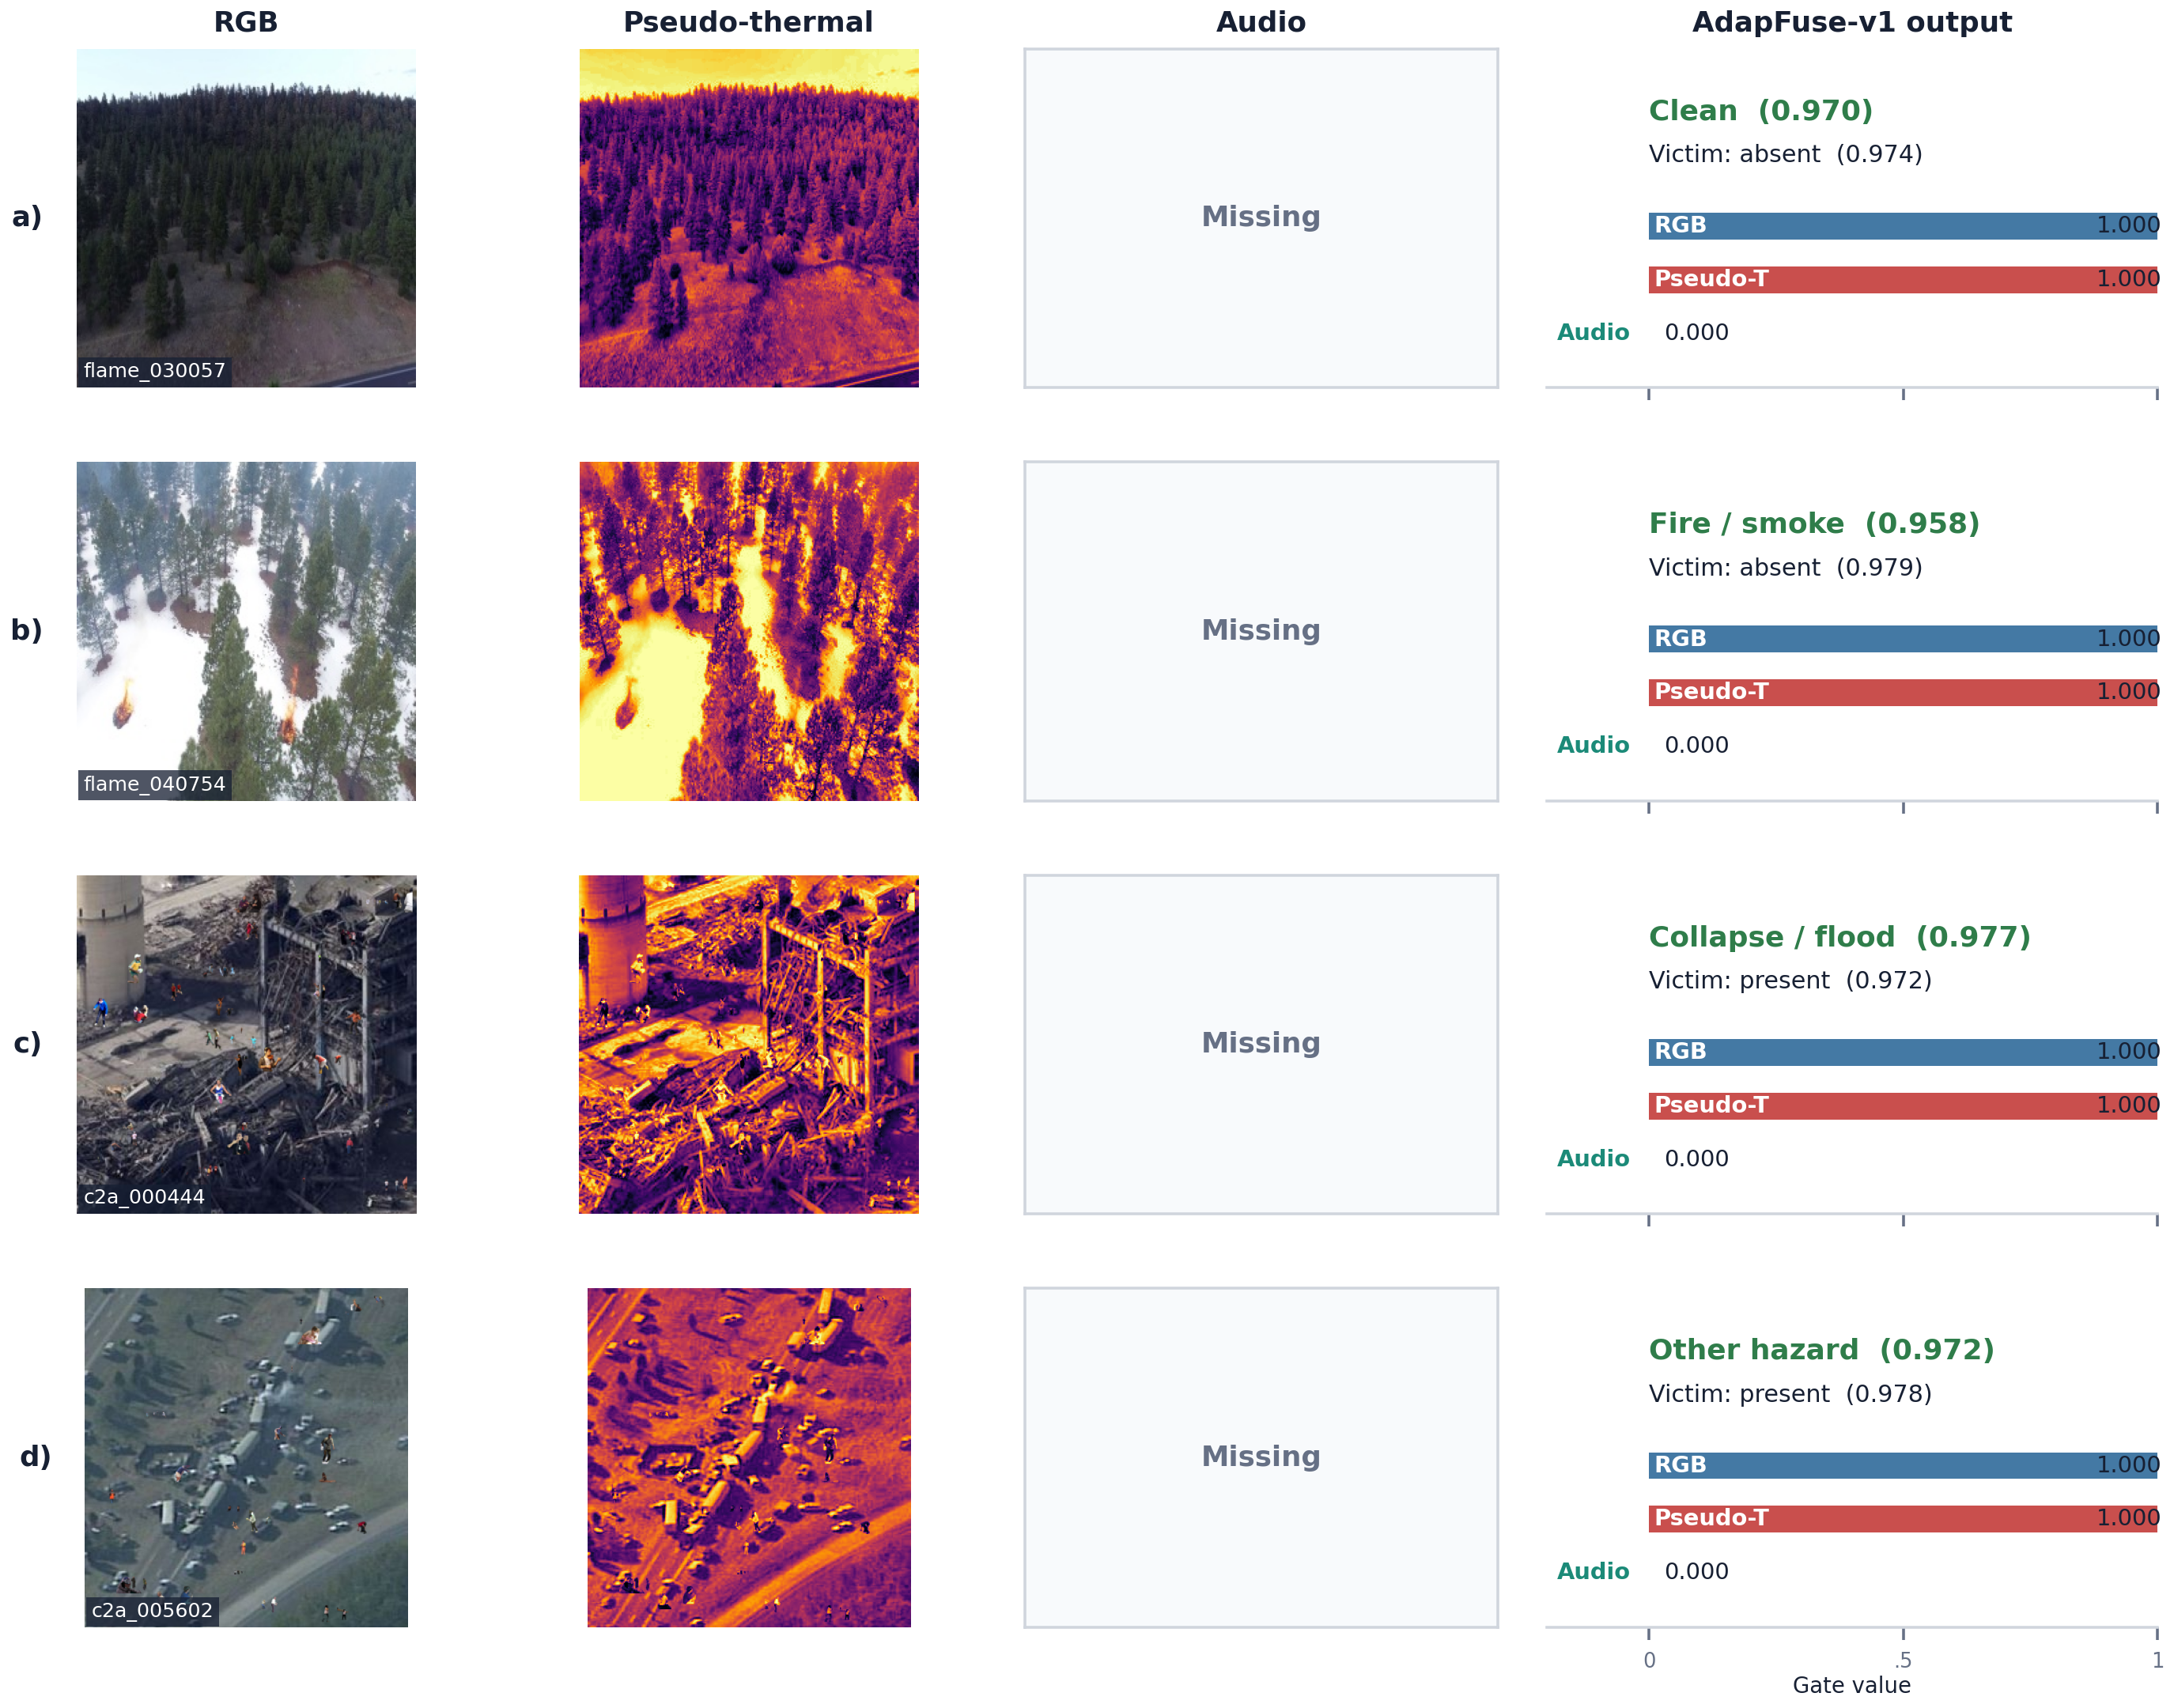
\includegraphics[width=\textwidth]{images/generated/fig_02_qualitative.png}
\caption{Four real held-out metadata rows and actual AdapFuse-v1 forward-pass outputs. Each row shows the source RGB image, its RGB-derived pseudo-thermal map, explicit absence of audio, predicted disaster and victim-presence classes, and reported modality gates. The model correctly classifies these four examples; the missing audio gate is forced to zero by the presence mask, while the two available image-derived streams saturate near one. All four rows are fixed entries of \texttt{test.csv} evaluated with a strict load of \texttt{adaptfuse\_v1\_best.pth}; none has an assigned audio clip, so the audio input is zero-filled and its presence flag is 0. These examples demonstrate missing-input execution, not synchronized tri-modal fusion.}
\label{fig:dataset_pipeline}
\end{figure}

\subsection{Dataset Split and Class Distribution}

\subsubsection{Raw Split and Class Imbalance}
\label{sec:dataset_split}

The 72{,}997 rows are split into train/validation/test by disaster-label stratification, producing 51{,}097 training, 10{,}949 validation, and 10{,}951 test rows. The split builder does not group by source video, flight, or near-duplicate sequence. Consequently, visually adjacent frames can occur across splits; the test set is held out at row level but is not a strict cross-flight generalization benchmark. A capture-group-aware split was subsequently constructed to measure the size of this effect; it is described and evaluated in Section~\ref{sec:grouped_split}, and all row-level scores in this work should be read alongside it. The raw training split is severely imbalanced: fire/smoke dominates at 46.5\% while collapse/flood and other hazards together account for only 12.5\%.

\subsubsection{Two-Stage Class Balancing}

To address this, a two-stage oversampling procedure is applied to the training and validation splits. The test set is \emph{never} resampled; it retains the natural distribution of the collection throughout all experiments.

\textbf{Stage 1: Disaster balance.} Each of the four disaster classes is oversampled to the majority-class count (23{,}746, the fire/smoke count) by sampling with replacement. All synthetic duplicate rows are marked with a synthetic-row indicator; the data loader applies stronger augmentation (additional jitter and masking) to these rows during training to reduce overfitting on duplicated samples.

\textbf{Stage 2: Victim balance.} After disaster balancing, the victim-present class (originally 21.7\% of training) is oversampled proportionally across disaster classes to achieve a 50/50 victim split while preserving the disaster class balance. This produces the \textit{full-balanced} split of 98{,}556 samples (48.2\% synthetic rows).

\subsubsection{Stratified Balanced Training Configuration (Resource Constraint)}

Training large suites of multimodal models on the full-balanced split ($\sim$98{,}556 samples) at batch size 16 on a single RTX 5090 (32\,GB VRAM) was estimated at planning time to require approximately 3 hours per run and $\sim$80 hours total. A \textit{Stratified Balanced Training Subset} is therefore derived by applying source-stratified 50\% sampling to each disaster class of the full-balanced split, with a minimum of 5 rows per dataset source to ensure no source is dropped. The result is exactly 12{,}319 rows per disaster class, halving the data per epoch while preserving exact class balance and full source coverage. (Actual logged run times, given below, were longer than this planning estimate.)

\textbf{All twenty-six trained multimodal classification models use the Stratified Balanced Training Configuration.} The grouped-split retraining of AdapFuse-v1 (Section~\ref{sec:grouped_split}) is a separate run outside these twenty-six and was trained without class balancing.

Table~\ref{tab:balancing} summarises the transformation from raw to final training distribution.

\begin{table}[H]
\centering
\caption{Dataset split transformation: raw $\to$ Stratified Balanced Subset (training and validation only; test set unchanged).}
\label{tab:balancing}
\resizebox{\textwidth}{!}{%
\begin{tabular}{@{}lrrrrrr@{}}
\toprule
& \multicolumn{2}{c}{\textbf{Raw (original)}} & \multicolumn{2}{c}{\textbf{Full balanced}} & \multicolumn{2}{c}{\textbf{Stratified Balanced (used)}} \\
\cmidrule(lr){2-3} \cmidrule(lr){4-5} \cmidrule(lr){6-7}
\textbf{Subset / Class} & \textbf{Count} & \textbf{\%} & \textbf{Count} & \textbf{\%} & \textbf{Count} & \textbf{\%} \\
\midrule
\textbf{Training total}         & 51{,}097 & n/a    & 98{,}556 & n/a    & \textbf{49{,}276} & n/a \\
\quad Normal / Clean (0)        & 20{,}959 & 41.0\% & 24{,}639 & 25.0\% & 12{,}319          & 25.0\% \\
\quad Fire / Smoke (1)          & 23{,}746 & 46.5\% & 24{,}639 & 25.0\% & 12{,}319          & 25.0\% \\
\quad Collapse / Flood (2)      &  4{,}355 &  8.5\% & 24{,}639 & 25.0\% & 12{,}319          & 25.0\% \\
\quad Other hazard (3)          &  2{,}037 &  4.0\% & 24{,}639 & 25.0\% & 12{,}319          & 25.0\% \\
\quad Victim present (of total) & 11{,}096 & 21.7\% & 49{,}278 & 50.0\% & 24{,}639          & 50.0\% \\
\quad Synthetic (augmented) rows&       0  &  0.0\% & 47{,}459 & 48.2\% & 23{,}696          & 48.1\% \\
\midrule
\textbf{Validation total}       & 10{,}949 & n/a    & 21{,}030 & n/a    & 10{,}516          & n/a \\
\textbf{Test total (held-out)}  & \multicolumn{6}{c}{10{,}951: natural distribution, never resampled} \\
\quad Normal (0)                & \multicolumn{6}{c}{4{,}492 (41.0\%) \quad Fire/Smoke (1): 5{,}089 (46.5\%) \quad Collapse (2): 934 (8.5\%) \quad Other (3): 436 (4.0\%)} \\
\bottomrule
\end{tabular}%
}
\footnotesize{Note: the Stratified Balanced training and validation totals (49{,}276 and 10{,}516) are each 1--2 rows short of an exact half of the full-balanced counts (98{,}556 and 21{,}030) due to per-source rounding under the minimum-5-rows-per-source constraint applied during stratified 50\% sampling.}
\end{table}

Figure~\ref{fig:dataset_composition} shows the source and label distributions for the dataset.

\begin{figure}[H]
\centering
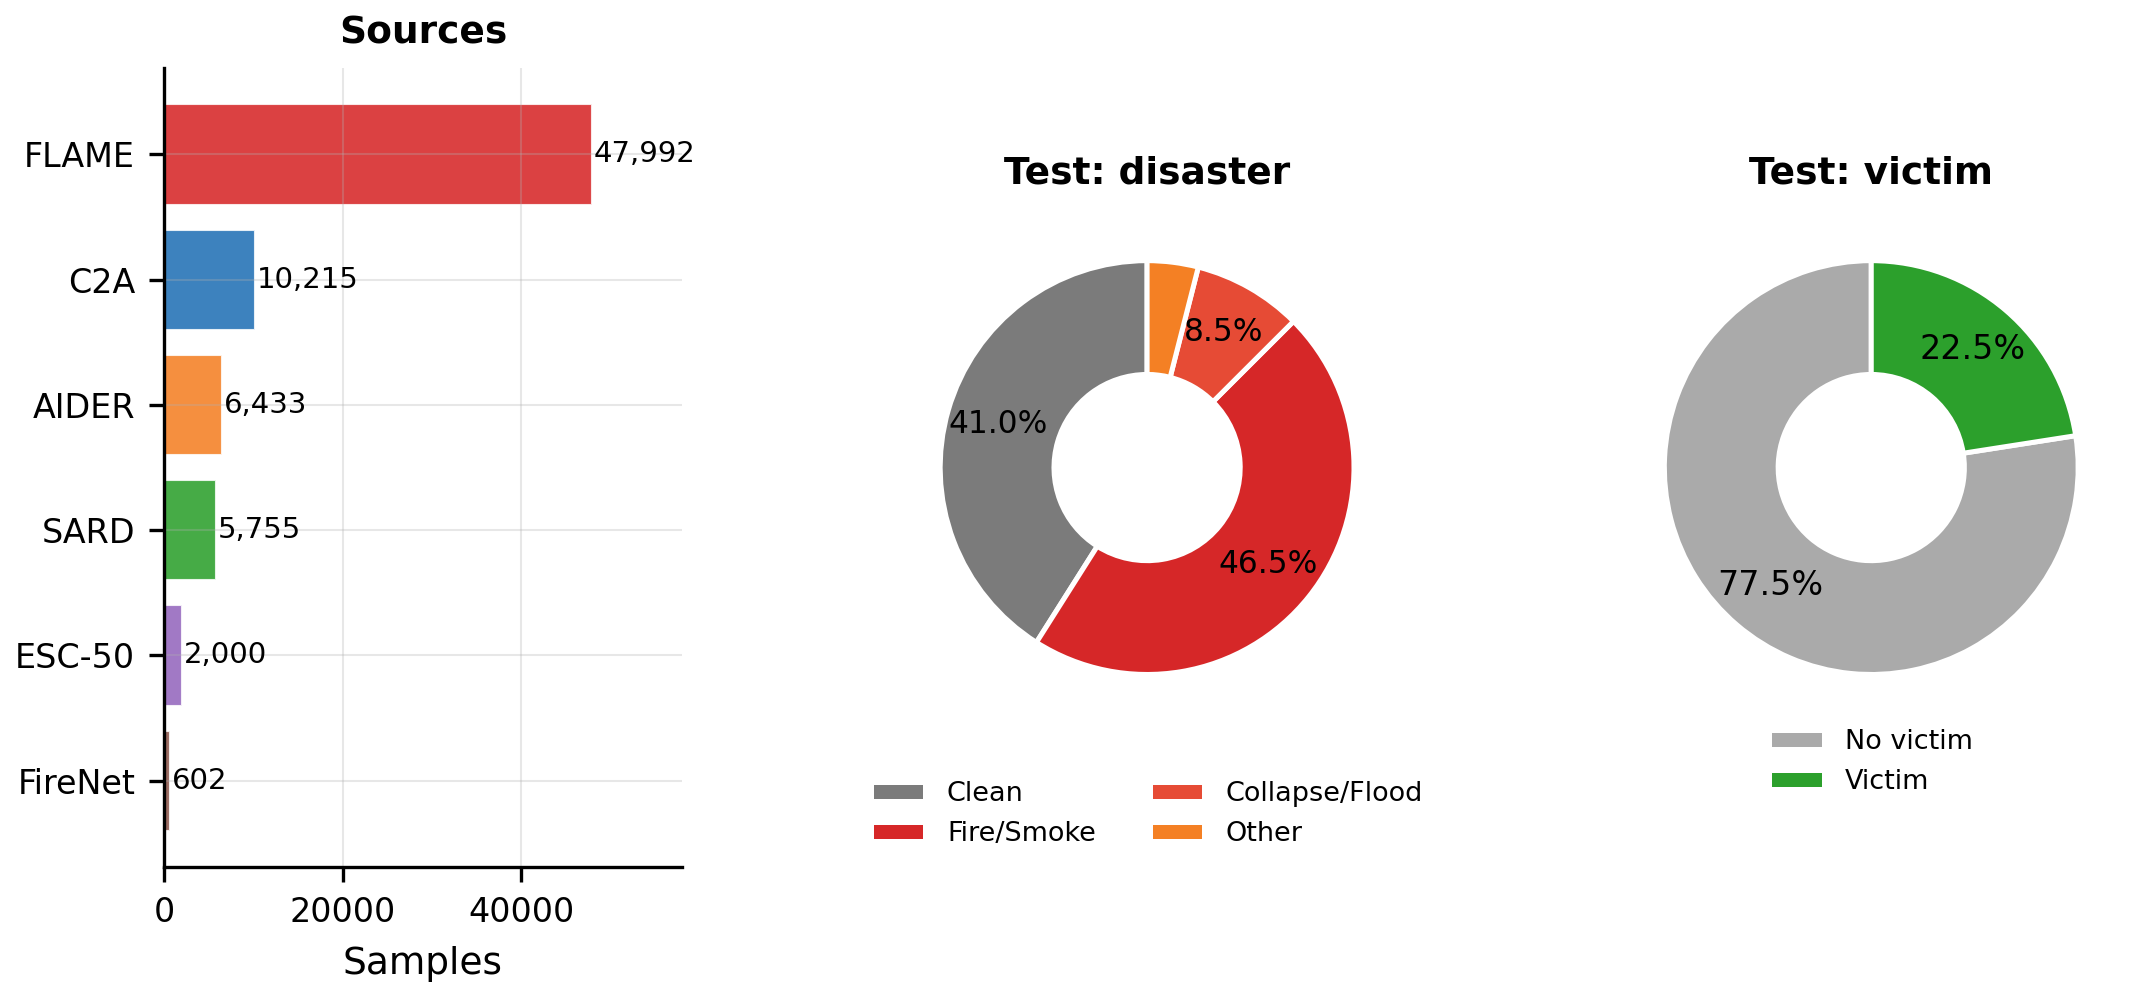
\includegraphics[width=\textwidth]{images/generated/fig_08_dataset.png}
\caption{Dataset composition: 72{,}997 samples from six public sources (left), and test-set label distributions for disaster class (centre) and victim detection (right). FLAME dominates at 65.7\% of all samples; the dataset is majority fire/smoke (46.5\% of test samples; other hazard 4.0\%) with 22.5\% victim-visible samples.}
\label{fig:dataset_composition}
\end{figure}

Figure~\ref{fig:balanced_training} visualises all four aspects of this transformation: disaster class redistribution, victim balance correction, per-source composition, and original-versus-synthetic row breakdown per class.

\begin{figure}[H]
\centering
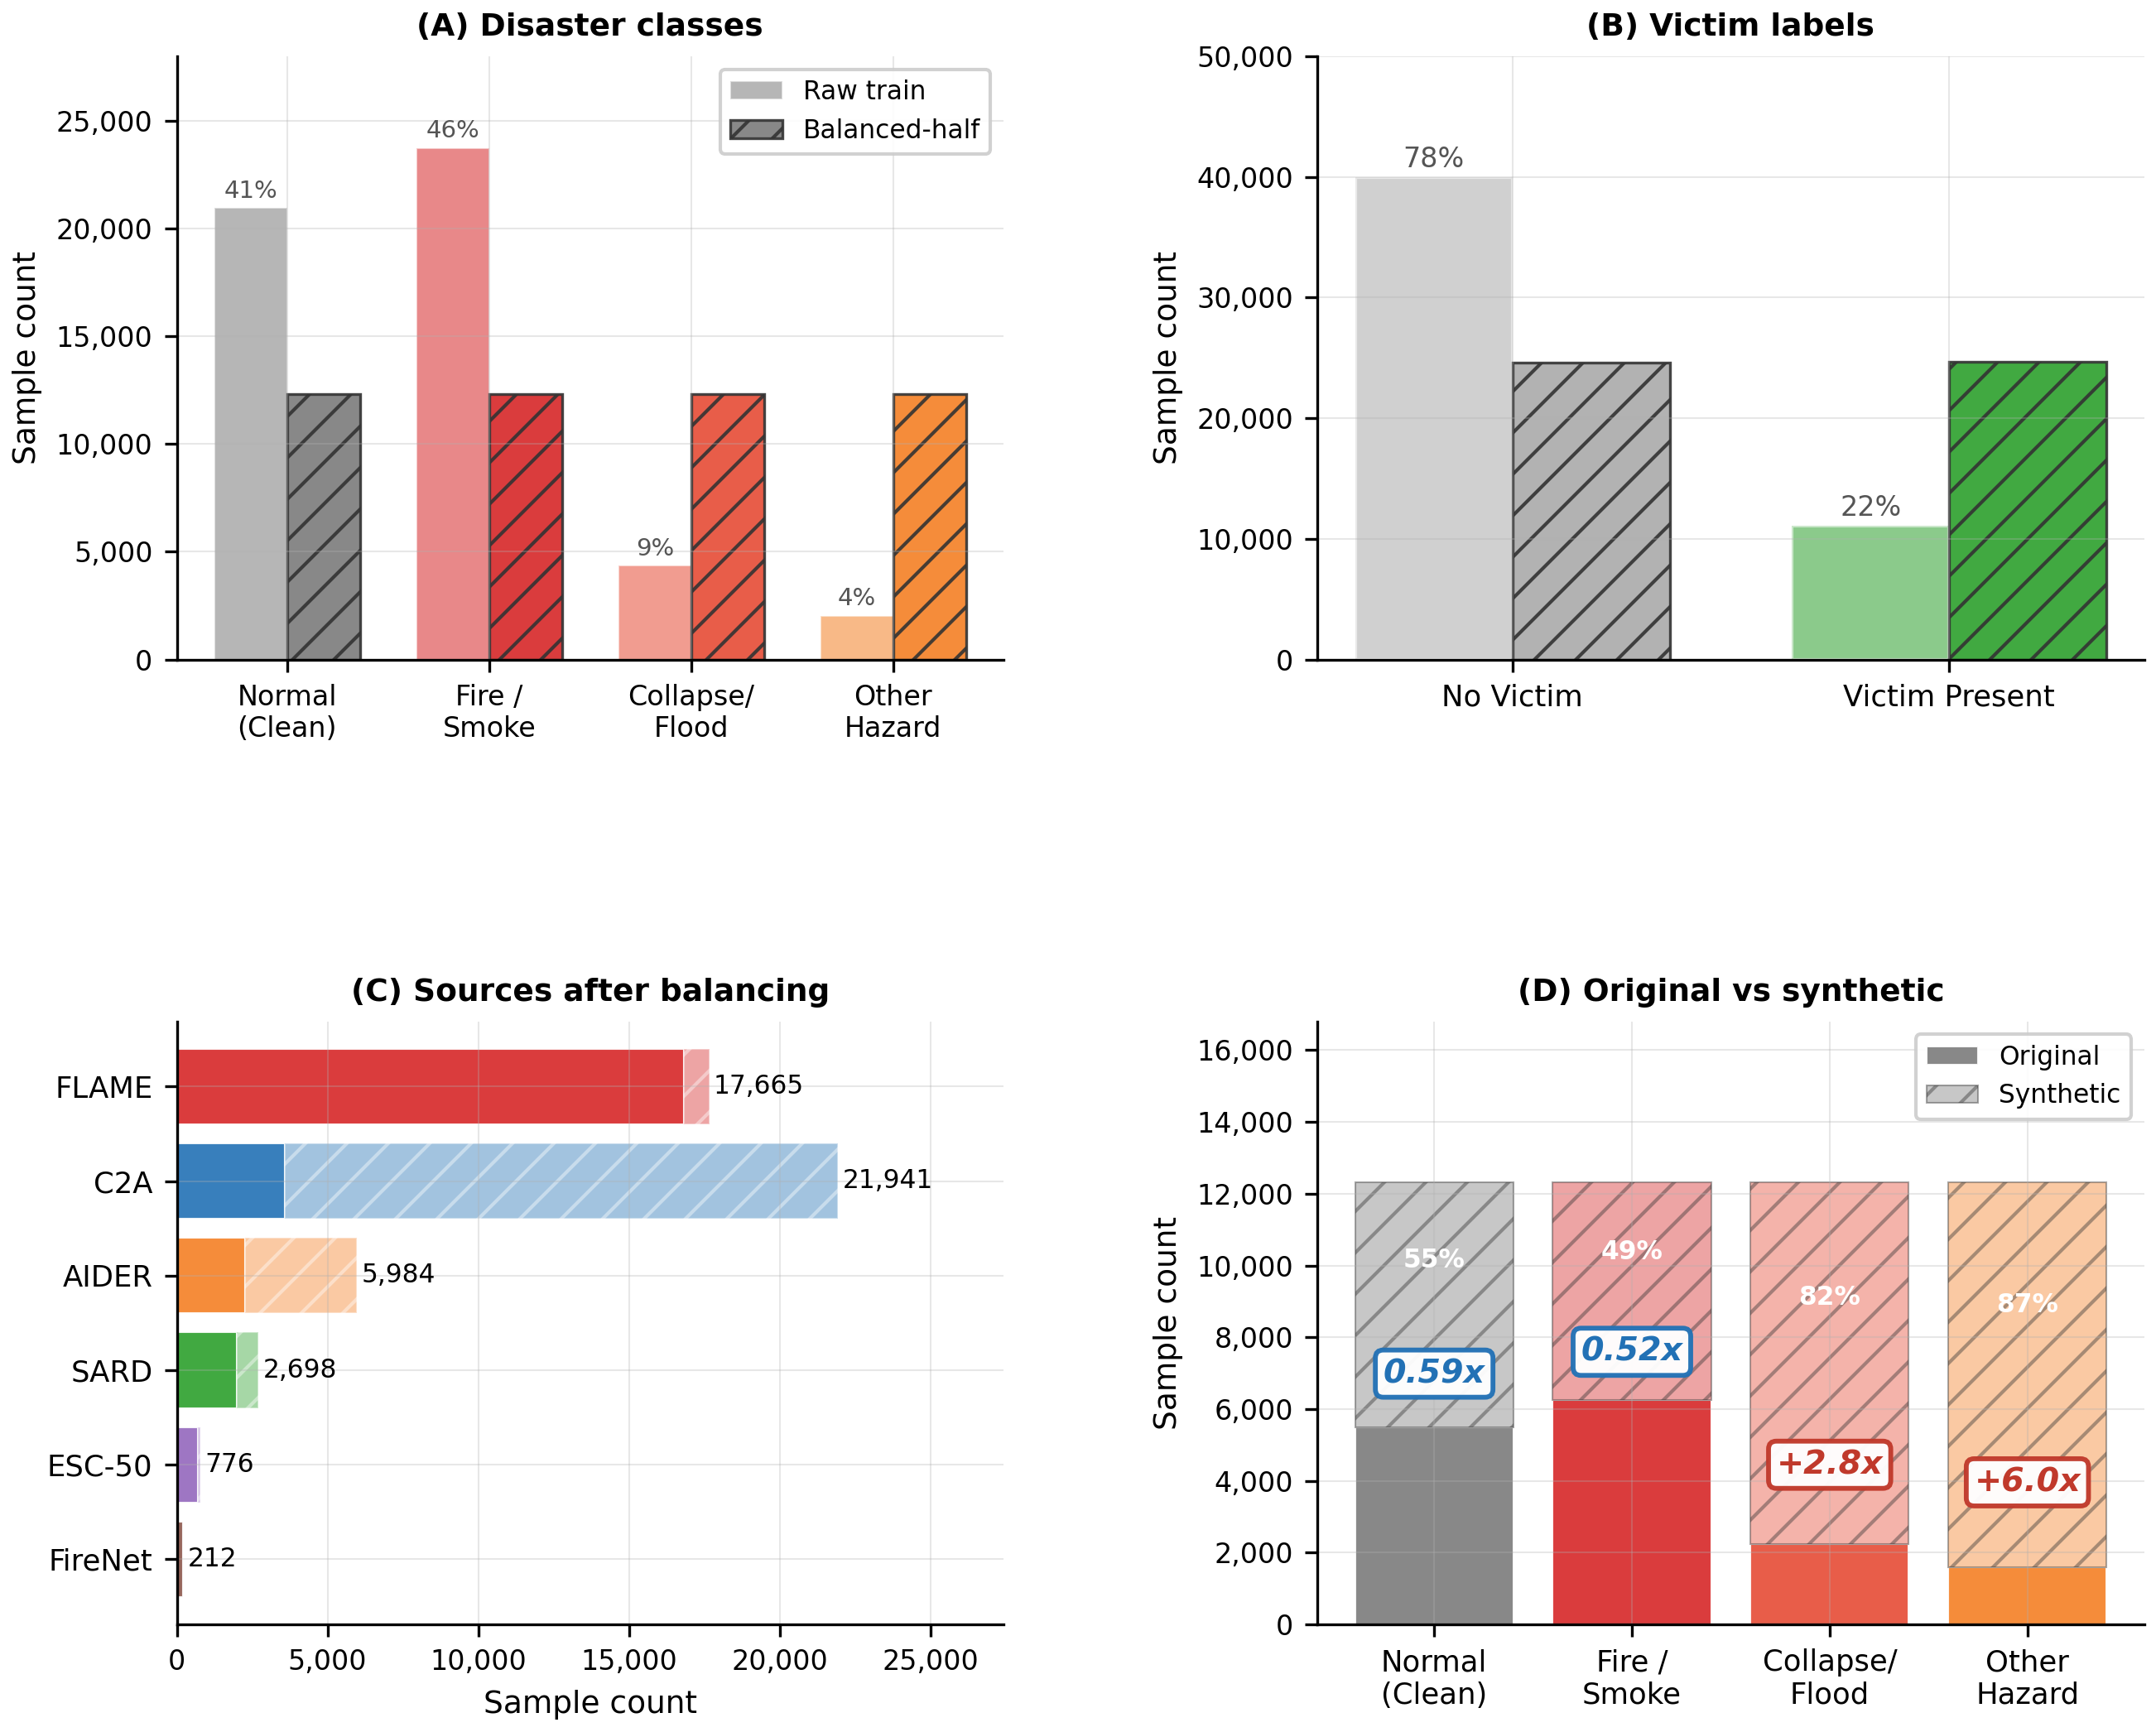
\includegraphics[width=\textwidth]{images/generated/fig_10_balanced_training.png}
\caption{Stratified Balanced Training Subset used across our trained multimodal models (49{,}276 samples: 12{,}319 per disaster class, 50/50 victim balance, 48.1\% synthetic rows). (A) Disaster class distribution: the raw training split is severely imbalanced (fire/smoke 46.5\%, other hazard 4.0\%); the stratified balanced subset achieves exact 25\% per class via two-stage oversampling. (B) Victim balance: raw 21.7\% victim-present corrected to 50/50. (C) Source composition in the 49{,}276-sample stratified balanced subset (solid: original rows, hatched: synthetic, as in D); all six sources are preserved. (D) Original vs synthetic (oversampled) rows per class: minority classes (collapse +2.8$\times$, other +6.0$\times$) are oversampled while majority classes (normal 0.59$\times$, fire 0.52$\times$) are effectively downsampled relative to the raw count; blue values indicate downsampling, red indicate oversampling, and percentages give the synthetic share of each class. All synthetic rows are marked as synthetic duplicates for stronger training augmentation.}
\label{fig:balanced_training}
\end{figure}

\noindent\textbf{Note on per-source composition.} C2A is the primary source for the Collapse/Flood and Other hazard classes, which are oversampled 2.8$\times$ and 6.0$\times$ respectively (Figure~\ref{fig:balanced_training}D) to reach the 12{,}319-per-class target. Because oversampling is applied at the class level rather than the source level, C2A's row count in the Stratified Balanced Training Subset (21{,}941) exceeds its entire raw sample count (10{,}215, Table~\ref{tab:dataset_sources}); this reflects heavy within-class duplication of C2A's minority-class rows, not an error in source accounting.

\noindent\textbf{Implication for metrics.} Because the test set retains the natural imbalanced distribution, \textit{macro F1} is reported as the primary metric throughout Chapter~5. Macro F1 weights each class equally regardless of frequency, correctly penalising a model that ignores the rare collapse/other classes. Accuracy (which weights by sample frequency) is reported as a secondary metric. The 8.5\% collapse and 4.0\% other classes together constitute only 12.5\% of test samples, meaning accuracy can remain above 98\% even when the model entirely fails on those classes.

\subsection{Data Preprocessing}

\textbf{RGB:} Images are resized to 224$\times$224 and normalized to ImageNet mean and standard deviation. The base training transform includes random horizontal flip, colour jitter, Gaussian blur, and rotation. Although the loader implements explicit smoke, low-light, motion-blur, and noise functions, the reported base configuration sets no \texttt{corruption\_type}; therefore its \texttt{corruption\_prob=0.3} does not activate those explicit corruptions. For reproducibility: every base training run reported in Chapter~5 (including Tables~\ref{tab:main_results}, \ref{tab:adaptfuse_extended} and \ref{tab:ablation_results}) used no synthetic corruption augmentation; the corruption sweeps appear only in the offline evaluation of Section~\ref{sec:robustness_stress_test}.

\textbf{Pseudo-thermal:} RGB-derived maps are read in grayscale, resized to 224$\times$224, and z-score normalized. The classification loader does not apply CLAHE in the reported AdapFuse-v1 run, and these intensity values are not radiometric temperatures.

\textbf{Audio:} Two-second clips at 16 kHz are transformed into normalized log-mel spectrograms (64 frequency bins, 63 time frames). The current classification loader does not apply spectral subtraction or SpecAugment. Rotor-noise corruption exists as an evaluation option but is not activated by the base training configuration without an explicit corruption type.

\textbf{Missing modality simulation:} During training, one sensor is randomly dropped (zero-filled) with probability 0.2 per sample, exposing each model to missing inputs during training.

\section{Preliminary Design: Six Fusion Architectures}

Six fusion designs are implemented and compared to evaluate the contribution of each design choice. Table~\ref{tab:designs} summarises the six designs; Figure~\ref{fig:design_comparison} illustrates the structural differences. For every design, including our own, the table lists the principal limitation observed in this study rather than only the intended benefit.

\begin{table}[H]
\centering
\caption{Summary of six fusion designs. \textit{Limitation} reports the main weakness of each design as observed in our experiments; the proposed designs (E, F) are assessed under the same criterion as the baselines.}
\label{tab:designs}
\resizebox{\textwidth}{!}{%
\begin{tabular}{@{}clp{4.6cm}p{5.2cm}@{}}
\toprule
\textbf{Design} & \textbf{Name} & \textbf{Approach} & \textbf{Limitation} \\
\midrule
A1 & RGB-only          & MobileNetV3-Small; 576-dim $\to$ FC classifier & No thermal or audio cue; fails in smoke/night \\
A2 & Thermal-only      & ResNet-18 (1-channel); 512-dim $\to$ FC classifier & No colour cue; lower spatial resolution \\
A3 & Audio-only        & 2D-CNN on log-mel (32$\to$64$\to$128 filters) & Label-matched ESC-50 clips; rotor noise not tested \\
B  & Early Fusion      & 5-channel input (RGB 3ch + Thermal 1ch + Audio resized 1ch) processed by one shared ResNet-18 & One backbone handles all sensor types; loses modality-specific features \\
C  & Late Fusion       & Three independent models produce class probabilities; learned weighted average & Sensors never share intermediate features \\
D  & Intermediate (Fixed) & Per-sensor backbone $\to$ 192-dim projection $\to$ concatenate $\to$ MLP & All sensors weighted equally regardless of quality \\
\midrule
E  & \textbf{AdapFuse-v1 (ours)} & Design D + RUE reliability weighting + cross-modal attention + NuisanceAwareHead & RUE gates unsupervised and saturated (static per-modality weights); single-step GRU; nuisance head unsupervised; only +0.05\,pp macro-F1 over D \\
F  & \textbf{AdapFuse-v2 (ours, KD)} & AdapFuse-v1 teacher $\to$ knowledge distillation $\to$ half-width student (proj\_dim=96) & Inherits all limitations of E; only 4.9\% fewer parameters (backbones unchanged); on-device latency not measured \\
\bottomrule
\end{tabular}%
}
\end{table}

\noindent Each unimodal baseline is also trained with two alternative backbones, giving three per modality: EfficientNet-B0 and MobileViT-XXS for RGB and for 1-channel pseudo-thermal, and a CNN6-style encoder and a GDBlock variant of the AudioCNN for audio. Section~\ref{sec:unimodal_backbones} reports these runs, which allow each fused model to be compared with a unimodal model that uses the same backbone.

\noindent\textbf{Limitations of the proposed designs.} Designs E and F are held to the same standard as the baselines. For AdapFuse-v1, three of its four added components do not yet behave as their names suggest. (i)~The RUE receives no degradation targets, so its gates converge to saturated, input-independent values and act as a learned static weighting per modality, not a dynamic reliability estimate (Section~\ref{sec:robustness_stress_test}). (ii)~The GRU runs on a sequence of length one and therefore provides no temporal smoothing. (iii)~The NuisanceAwareHead receives no nuisance labels, so its loss is zero during training. The measured gain over the fixed-weight Design D is correspondingly small: +0.05\,pp combined macro-F1, together with a 2.9$\times$ lower focal test loss (Figure~\ref{fig:design_comparison}). AdapFuse-v2 inherits these properties. Because distillation halves only the projection width while the backbones stay unchanged, it removes just 4.9\% of the parameters (12.94M $\to$ 12.30M), and its deployment benefit has not been verified on embedded hardware. Accordingly, we present E and F as an architecture whose adaptive components are \emph{implemented but not yet validated}. Sections~\ref{sec:robustness_stress_test} and~\ref{sec:grouped_gates} give the supporting evidence, and the concluding chapter outlines the supervision needed to validate them.

\begin{figure}[H]
\centering
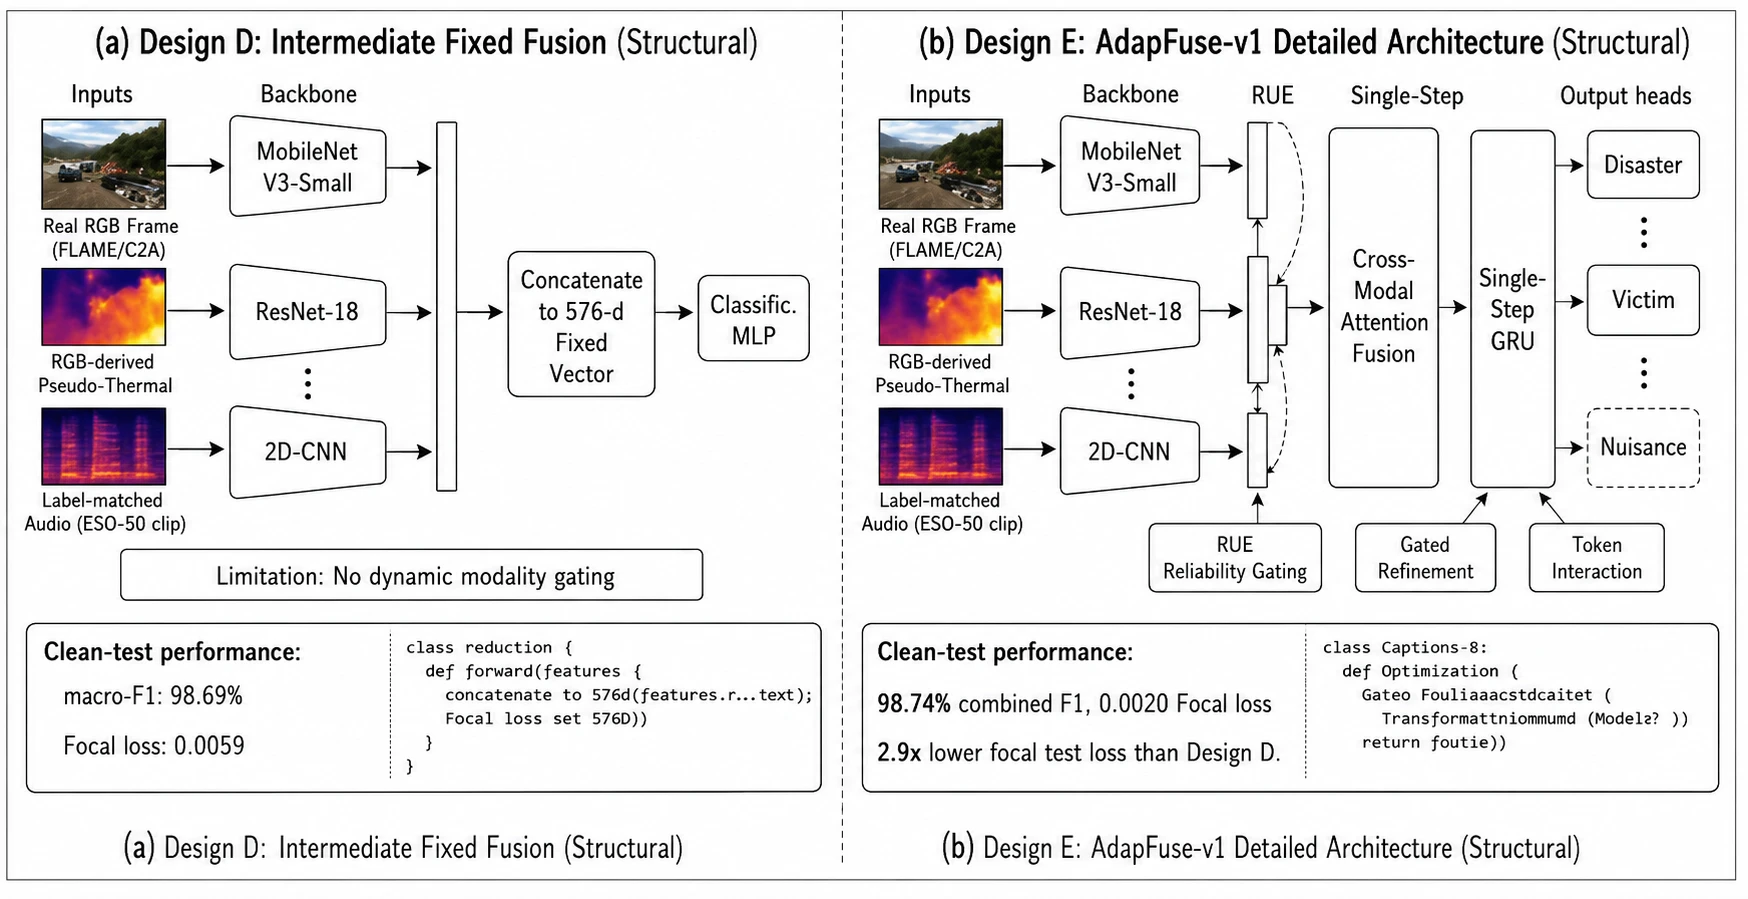
\includegraphics[width=\textwidth]{images/generated/4.5.png}
\caption{Structural and measured clean-test comparison of Design D and Design E. AdapFuse-v1 improves combined macro-F1 by 0.05 percentage points and lowers the reported focal test loss by 2.9$\times$. Its GRU is single-step in the current loader; the nuisance branch is present but unsupervised because \texttt{nuisance\_gt} is not supplied. The diagram therefore separates implemented structure from demonstrated effect.}
\label{fig:design_comparison}
\end{figure}

Figure~\ref{fig:data_provenance} summarises what our metadata actually supply for each modality, and which supervision signals assumed by the architecture are absent from it.

\begin{figure}[H]
\centering
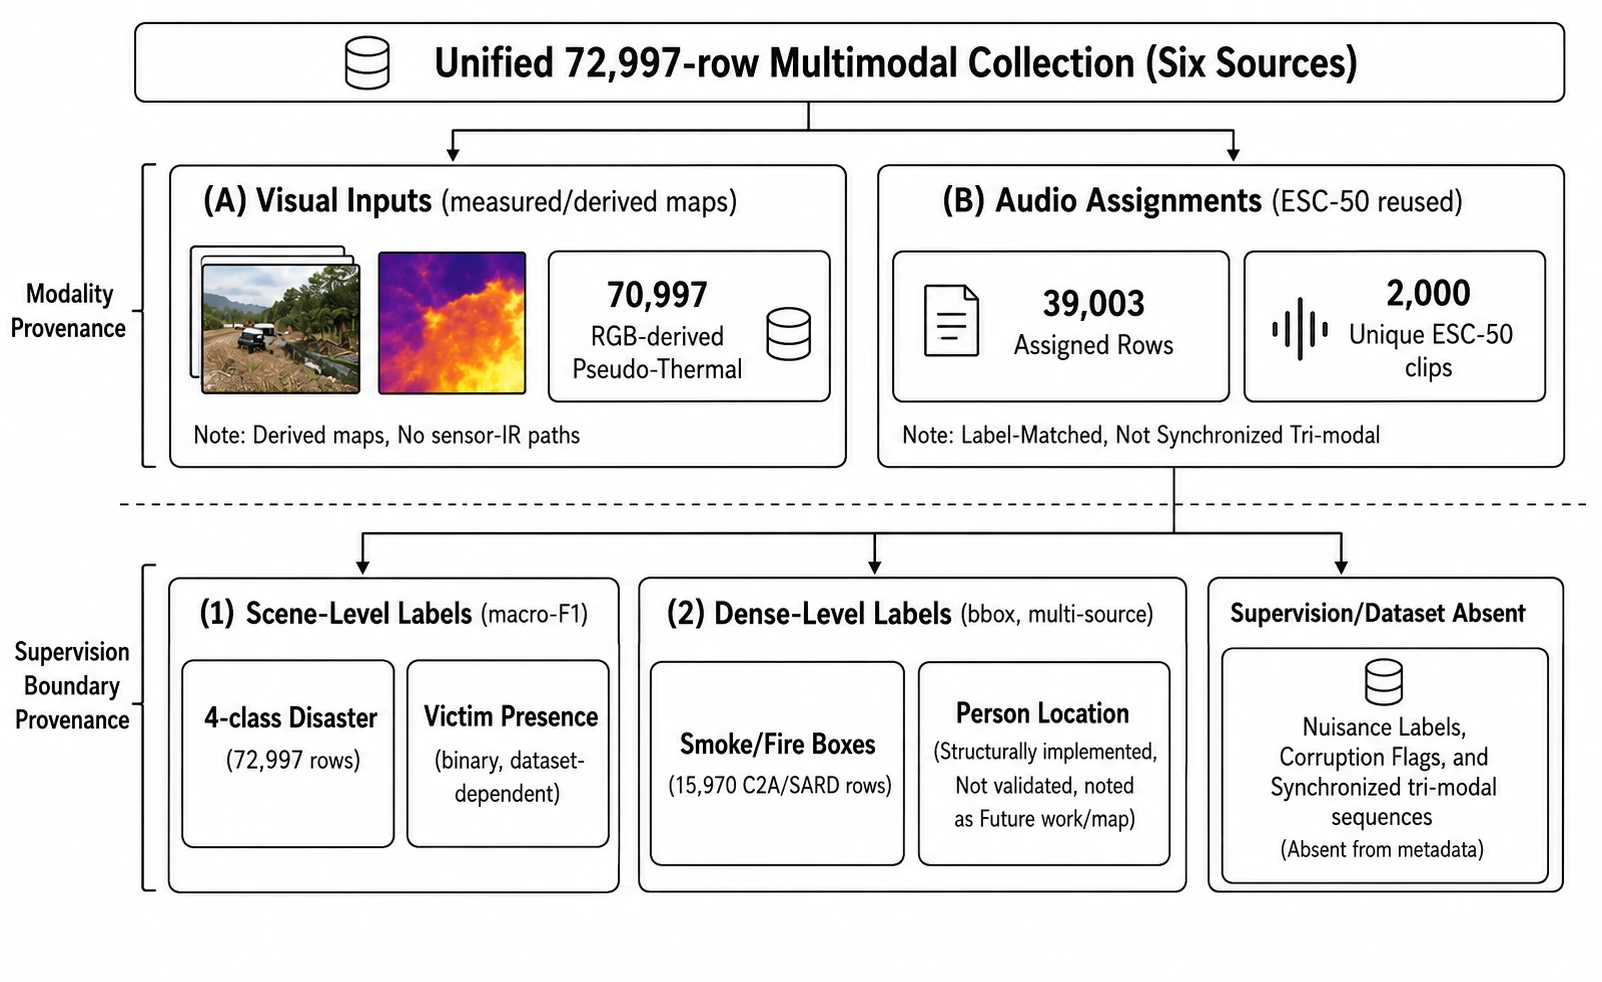
\includegraphics[width=\textwidth]{images/generated/4.6.png}
\caption{Data provenance and supervision boundary recomputed from our metadata. The unified collection contains 70{,}997 measured RGB images, 70{,}997 RGB-derived pseudo-thermal maps, and 39{,}003 audio assignments referencing 2{,}000 unique ESC-50 clips. Bounding-box paths occur in 15{,}970 C2A/SARD rows. Nuisance labels, corruption flags, sensor-IR frames, and synchronized tri-modal sequences are absent.}
\label{fig:data_provenance}
\end{figure}

\section{AdapFuse-v1: Detailed Architecture}

\subsection{Modality-Specific Encoders}

Each sensor has a dedicated lightweight backbone producing a 192-dimensional projected feature:

\begin{itemize}
    \item \textbf{RGB:} MobileNetV3-Small~\cite{howard2019mobilenetv3} pretrained on ImageNet. The 576-dim pooled output of its final $1\times1$ convolution is projected to 192 dimensions via a linear layer. Compute: $\approx$0.06 GMACs per frame (Table~\ref{tab:backbone_candidates}).
    \item \textbf{Pseudo-thermal:} ResNet-18~\cite{he2016deep} adapted for single-channel input (pretrained first-layer weights summed across the RGB channels). The 512-dim global average-pooled output is projected to 192 dimensions. All populated thermal paths in our metadata are RGB-derived maps; no sensor-IR inputs are evaluated.
    \item \textbf{Audio:} A three-layer 2D-CNN on the 64$\times$63 log-mel spectrogram (filter progression 32$\to$64$\to$128). Global average pooling produces a 128-dim vector projected to 192 dimensions.
\end{itemize}

Each backbone additionally outputs a 16-dimensional \textit{quality token}, a learned linear projection of its penultimate activations intended to summarise how distinctive and high-confidence the backbone's internal representation is.

\subsection{Reliability and Uncertainty Estimator (RUE)}

The RUE is a two-layer MLP that receives the three 16-dim quality tokens plus a 6-dim vector of feature statistics (per-modality mean and variance of the 192-dim features). It outputs three sigmoid gates $r_i \in [0,1]$ and three uncertainty values. In the reported training path, degradation targets are passed as \texttt{None}; the gates are therefore shaped indirectly by task loss and a variance regularizer rather than calibrated against sensor-quality ground truth:

\begin{equation}
    [r_{rgb}, r_{th}, r_{au}] = \sigma\!\left(W_2 \cdot \text{ReLU}(W_1 \cdot [\mathbf{q}_{rgb}\|\mathbf{q}_{th}\|\mathbf{q}_{au}\|\mathbf{s}] + b_1) + b_2\right)
\end{equation}

where $\mathbf{q}_i \in \mathbb{R}^{16}$ are quality tokens, $\mathbf{s} \in \mathbb{R}^6$ are feature statistics, and $\sigma$ is the sigmoid function. Each modality's 192-dim feature vector is multiplied by its reliability score before entering the attention module, so that, by design, a modality with a low gate contributes less to the fused representation.

\textbf{Limitation.} Because no degradation labels or corruption flags are supplied (\texttt{degradation\_targets=None}), nothing in training ties a gate value to sensor quality. In our row-level model, the RGB and pseudo-thermal gates are saturated at $\approx$1.0 on every row that has the input and the audio gate is $\approx$0.011, and none of them moves across the synthetic corruption sweeps (Section~\ref{sec:robustness_stress_test}); the grouped-split retraining converges to different, equally saturated gates (Section~\ref{sec:grouped_gates}). The RUE therefore acts in these experiments as a learned, run-dependent on/off weighting per modality, not as a dynamic reliability estimator. Supervising it with explicit degradation targets and testing gate response against measured degradation is future work.

\subsection{Cross-Modal Attention Fusion}

The three reliability-weighted features are stacked as tokens $\mathbf{T} \in \mathbb{R}^{3 \times 192}$ and processed by a multi-head cross-attention module~\cite{vaswani2017attention} with 4 heads. This allows each modality to attend to context from the other two, learning complementary cross-sensor patterns (e.g.\ RGB flame-region attending to the thermal hotspot token):

\begin{equation}
    \hat{\mathbf{T}} = \text{MultiHead}(\mathbf{T}, \mathbf{T}, \mathbf{T})
\end{equation}

The mean-pooled output $\hat{f} = \text{mean}(\hat{\mathbf{T}}) \in \mathbb{R}^{192}$ is passed through a GRU (hidden size 192). The current dataset provides independent frames and the implementation calls the GRU on \texttt{fused.unsqueeze(1)} without passing a hidden state, so sequence length is one and each sample starts from a zero state; nothing is carried between frames. It is therefore a gated nonlinear refinement layer in these experiments; temporal smoothing across frames is not evaluated.

\subsection{NuisanceAwareHead}

The NuisanceAwareHead defines logits for:
\begin{enumerate}
    \item \textbf{Disaster class} (0=clean, 1=fire/smoke, 2=collapse/flood, 3=other), the primary task
    \item \textbf{Victim presence} (binary), the secondary task
    \item \textbf{Nuisance type} (5-class: clean signal, solar heating, RGB false fire, audio false alarm, partial occlusion), an architectural auxiliary branch
\end{enumerate}

In our trainer, \texttt{nuisance\_gt=None}; consequently the nuisance loss is zero and this branch is not supervised in the reported checkpoints. At inference only disaster and victim logits are reported. The observed false-positive rate must therefore be attributed to the trained scene classifier as a whole, not specifically to nuisance supervision. Our dataset contains no nuisance-category labels, so the nuisance branch is an unvalidated architectural provision rather than a demonstrated contribution; validating it would require nuisance-labelled false-alarm data and a comparison of false-positive rates with and without nuisance supervision.

\subsection{Visual and Audio Backbone Variants}

In addition to the baseline encoders, several architectural variants were implemented:
\begin{itemize}
    \item \textbf{EfficientNet-B0 Visual Backbones:} Replacing MobileNetV3-Small or ResNet-18 with EfficientNet-B0~\cite{tan2019efficientnet}, which leverages compound scaling across network depth, width, and resolution to capture fine-grained spatial and thermal signatures.
    \item \textbf{MobileViT-XXS Hybrid Transformer:} Incorporating MobileViT-XXS~\cite{mehta2022mobilevit}, combining MobileNet inverted residual blocks with lightweight Transformer self-attention to capture long-range aerial disaster scene dependencies at a small parameter budget (edge-device memory use is not measured here).
    \item \textbf{PANNS-CNN6-style Audio Backbone:} A 4-block convolutional network with the channel widths of PANNs CNN6~\cite{kong2020panns} (64--512), producing 512-dimensional acoustic representations. Our implementation uses $3\times3$ kernels, whereas the released AudioSet checkpoint uses $5\times5$ kernels, so none of the checkpoint's convolution weights load (only 8 of 20 tensors, all batch-normalisation parameters). This encoder is therefore effectively trained from scratch, not an AudioSet transfer.
    \item \textbf{AudioCNN-GD Backbone:} A multi-scale dilated convolutional architecture employing parallel dilation rates ($d \in \{1, 3, 5\}$) to capture both transient bursts and sustained frequency patterns, a design aimed at rotor-noise environments (not tested here with measured rotor noise).
\end{itemize}

\subsection{Backbone Selection Rationale}
\label{sec:backbone_selection}

The encoders were chosen against four criteria derived from the target payload (Section~\ref{sec:tech_requirements}: embedded GPU with TDP $\leq$15\,W, $\geq$10 FPS, INT8 inference for all encoders):
\begin{enumerate}
    \item \textbf{Pretrained weights.} Each visual encoder must have public ImageNet weights, and the audio encoder should have AudioSet weights, because every training source is small relative to these corpora.
    \item \textbf{Per-stream compute budget.} Three encoders run on every frame, so each is limited to about 1\,GMAC and 5\,M parameters at $224\times224$. This budget is a design choice, not a measured limit of a specific edge device.
    \item \textbf{Accuracy within the budget.} Among candidates inside the budget, those with the highest ImageNet top-1 are preferred.
    \item \textbf{Family diversity.} The three visual candidates cover three design families (a hand-designed mobile CNN, a compound-scaled CNN and a CNN--Transformer hybrid), so a backbone ablation tests different inductive biases, not three sizes of one network.
\end{enumerate}

Table~\ref{tab:backbone_candidates} applies these criteria to thirteen visual candidates. Parameters, MACs and training memory were measured by us with a single benchmark script; ImageNet top-1 is the value published with each set of weights. These quantities are properties of each network rather than of the GPU. Latency on the RTX 5090 (32\,GB VRAM) training workstation would not predict on-board UAV latency, so it is not used as a selection criterion.

\begin{table}[H]
\centering
\caption{Visual backbone candidates. Params and MACs are for the feature extractor without its ImageNet classifier, at a $3\times224\times224$ input. Train memory is PyTorch peak allocated memory for one mixed-precision forward--backward--AdamW step of the backbone alone at batch 16. Shaded rows are inside the per-stream budget ($\leq$1\,GMAC, $\leq$5\,M params). $^\dagger$Lower bound: fused attention kernels are not counted. $^\ddagger$From the torchvision weights metadata, because the counter misses fused attention. $^\ast$Pseudo-thermal A2 only; over budget (see text). Top-1: ImageNet; Mem.: training memory.}
\label{tab:backbone_candidates}
\resizebox{\textwidth}{!}{%
\begin{tabular}{@{}llcccc l@{}}
\toprule
\textbf{Backbone} & \textbf{Family} & \textbf{Params (M)} & \textbf{GMACs} & \textbf{Top-1 (\%)} & \textbf{Mem.\ (MB)} & \textbf{Decision} \\
\midrule
\rowcolor{gray!12} MobileNetV3-Small~\cite{howard2019mobilenetv3} & Mobile CNN & 0.93 & 0.06 & 67.7 & 151 & \textbf{Selected} \\
\rowcolor{gray!12} ShuffleNetV2-1.0$\times$ & Mobile CNN & 1.25 & 0.14 & 69.4 & 194 & Not used \\
\rowcolor{gray!12} MobileNetV3-Large~\cite{howard2019mobilenetv3} & Mobile CNN & 2.97 & 0.21 & 74.0 & 404 & Not used \\
\rowcolor{gray!12} MobileNetV2 & Mobile CNN & 2.22 & 0.30 & 71.9 & 655 & Not used \\
\rowcolor{gray!12} MobileViT-XXS~\cite{mehta2022mobilevit} & Hybrid & 0.95 & 0.30$^\dagger$ & 69.0 & 414 & \textbf{Selected} \\
\rowcolor{gray!12} EfficientNet-B0~\cite{tan2019efficientnet} & Scaled CNN & 4.01 & 0.39 & 77.7 & 779 & \textbf{Selected} \\
EfficientNet-B3~\cite{tan2019efficientnet} & Scaled CNN & 10.70 & 0.96 & 82.0 & 1{,}546 & Over (params) \\
MobileViT-S~\cite{mehta2022mobilevit} & Hybrid & 4.94 & 1.52$^\dagger$ & 78.4 & 1{,}218 & Over (MACs) \\
ResNet-18~\cite{he2016deep} & CNN & 11.18 & 1.81 & 69.8 & 451 & \textbf{Selected}$^\ast$ \\
ResNet-50~\cite{he2016deep} & CNN & 23.51 & 4.09 & 76.1 & 1{,}152 & Over (MACs) \\
ConvNeXt-Tiny & CNN & 27.82 & 4.46 & 82.5 & 1{,}450 & Over (MACs) \\
Swin-T & ViT & 27.52 & 4.49 & 81.5 & 1{,}591 & Over (MACs) \\
ViT-B/16 & ViT & 85.80 & 17.56$^\ddagger$ & 81.1 & 2{,}628 & Over (MACs) \\
\bottomrule
\end{tabular}%
}
\end{table}

\textbf{Visual encoders.} MobileNetV3-Small is the cheapest candidate (0.06\,GMACs) and is the default RGB encoder of every fused model. EfficientNet-B0 has the highest ImageNet accuracy inside the budget (77.7\%), and MobileViT-XXS is the only CNN--Transformer hybrid inside it. The other in-budget candidates were not trained: each costs more MACs than MobileNetV3-Small and has a lower top-1 than EfficientNet-B0, so it lies inside the cost--accuracy range the three selected networks already cover. Every candidate above 1\,GMAC was rejected; the larger models (ResNet-50, ConvNeXt-Tiny, Swin-T, ViT-B/16) need 4--18$\times$ the budget per stream while gaining at most 4.8 top-1 points over EfficientNet-B0.

\textbf{Pseudo-thermal encoder.} ResNet-18 is the exception: at 1.81\,GMACs and 11.2\,M parameters it is over budget. It was kept as the A2 baseline because single-channel adaptation of a pretrained ResNet by summing first-layer weights is a common transfer baseline for grey-scale and thermal imagery. The two in-budget replacements are tested directly: both EfficientNet-B0 and MobileViT-XXS outperform it on the pseudo-thermal stream with 2.8--11.8$\times$ fewer parameters (Table~\ref{tab:unimodal_thermal}).

\begin{table}[H]
\centering
\caption{Audio backbone candidates at the $1\times64\times63$ log-mel input. Upper rows are measured by the same script as Table~\ref{tab:backbone_candidates}. Lower rows are reported by Kong et al.~\cite{kong2020panns} for the full networks at their own input size, including the classifier, and are shown for scale.}
\label{tab:audio_candidates}
\resizebox{\textwidth}{!}{%
\begin{tabular}{@{}lccccl@{}}
\toprule
\textbf{Backbone} & \textbf{Params (M)} & \textbf{GMACs} & \textbf{AudioSet mAP} & \textbf{Train mem.\ (MB)} & \textbf{Decision} \\
\midrule
AudioCNN (from scratch) & 0.09 & 0.037 & -- & 48 & \textbf{Selected} \\
AudioCNN + GDBlock & 0.06 & 0.022 & -- & 58 & \textbf{Selected} \\
CNN6-style encoder ($3\times3$)$^\ast$ & 1.55 & 0.213 & -- & 102 & \textbf{Selected} \\
\midrule
PANNs CNN6 (reported)~\cite{kong2020panns} & 4.8 & -- & 0.343 & -- & Reference \\
PANNs CNN10 (reported)~\cite{kong2020panns} & 5.2 & -- & 0.380 & -- & Over (params) \\
PANNs CNN14 (reported)~\cite{kong2020panns} & 80.8 & -- & 0.431 & -- & Over (params) \\
\bottomrule
\multicolumn{6}{@{}l}{\footnotesize $^\ast$Intended as PANNs CNN6 transfer, but the AudioSet convolution weights ($5\times5$) do not match its $3\times3$ kernels and are not loaded.}
\end{tabular}%
}
\end{table}

\textbf{Audio encoders.} The three audio encoders cover training from scratch (AudioCNN), a cheaper multi-scale variant (GDBlock) and a wider CNN6-style encoder. The CNN6-style encoder was meant to test AudioSet transfer, but because of the kernel mismatch described above it was trained without pretrained convolution weights, so this thesis does not test AudioSet transfer. Larger audio networks such as PANNs CNN14 are about 16 times over the parameter budget. Because the audio in this corpus is label-matched ESC-50 rather than synchronised UAV audio, a larger audio encoder would not address the main limitation of the audio stream (Section~\ref{sec:unimodal_backbones}).

\textbf{Scope of the selection.} This procedure selects backbones by cost and published accuracy. The selected backbones were then trained end-to-end inside the AdapFuse-UAV training pipeline, not benchmarked as stand-alone ImageNet classifiers: each was trained as the encoder of a unimodal baseline (Section~\ref{sec:unimodal_backbones}) and as an encoder of AdapFuse-v1 (Section~\ref{sec:backbone_variants}), with the same data loader, class balancing, augmentation, focal loss, mixed precision, early stopping and evaluation as every other model (no synthetic corruption was applied during training). Candidates that were not selected were not trained, so the thesis does not show that they would perform worse on this corpus.

\subsection{Architectural Augmentations and Component Ablations}

\begin{itemize}
    \item \textbf{Spatial Attention Gating:} Modifies the fusion bottleneck by maintaining 2D spatial feature grids ($7 \times 7$) from RGB and thermal backbones before pooling, applying cross-modal spatial attention to align visual smoke plumes with thermal hotspots prior to RUE confidence weighting.
    \item \textbf{Domain Prompt Tokens:} Introduces $K=4$ learnable condition prompt vectors that interact with modality tokens via self-attention to encode environmental priors (e.g., daytime vs. night-time, clear vs. smoke-obscured flight).
    \item \textbf{Isolated Component Ablation Models:} Five diagnostic variants systematically omitting or replacing key architectural blocks: (1) \texttt{ablation\_no\_gru} (omitting the single-step GRU refinement); (2) \texttt{ablation\_no\_attention} (replacing 4-head attention with mean pooling); (3) \texttt{ablation\_no\_quality\_tokens} (stripping learned quality heads); (4) \texttt{ablation\_no\_nuisance} (disabling the defined but unsupervised nuisance head); and (5) \texttt{ablation\_no\_rue} (enforcing uniform unweighted fusion).
\end{itemize}

\subsection{Unified Multi-Task Architecture: UniAdapFuse}
\label{sec:uniadaptfuse_arch}

To bridge global scene perception with dense localized hazard detection, \textbf{UniAdapFuse} integrates a dual-stream architecture sharing multi-scale visual features:
\begin{enumerate}
    \item \textbf{Multi-Scale Feature Pyramid:} High-resolution intermediate feature maps ($C_2, C_3, C_4, C_5$) are extracted from RGB and Thermal backbones and merged via lateral connections to build a unified Feature Pyramid Network (FPN).
    \item \textbf{Cross-Scale Bidirectional Bridges:}
    \begin{itemize}
        \item \textit{Top-Down Context Gate (TDCG):} The fused global latent scene representation and RUE reliability scores modulate multi-scale detection features via Feature-wise Linear Modulation (FiLM)~\cite{perez2018film}, with the aim of suppressing false candidate boxes in clean scenes. This effect is not validated, because the joint detector records $\mathrm{mAP}_{50}=0.0$ (Section~\ref{sec:uniadaptfuse}).
        \item \textit{Bottom-Up Spatial Guidance (BUSG):} Aggregated bounding-box saliency maps from the detection head are pooled to enrich the victim localization classifier.
    \end{itemize}
    \item \textbf{Gradient Isolation and Phased Curriculum:}
    To reduce multi-task negative transfer, where dense bounding box gradients may disturb the shared classification backbone, UniAdapFuse v2 changes the following relative to the naive v1 run:
    \begin{itemize}
        \item \textit{Phased Curriculum:} Training begins with Phase~1 (15 epochs) freezing the detection neck and head to establish robust classification representations, followed by Phase~2 joint training.
        \item \textit{Stop-Gradient Isolation:} Pyramid features entering the detection neck are detached (\texttt{.detach()}), preventing bounding-box regression loss from overwriting shared perceptual features.
        \item \textit{Differentiated Learning Rates:} Backbone encoders are updated with $0.1\times$ base learning rate ($5.0 \times 10^{-5}$), the classification stream at $1.0\times$ ($5.0 \times 10^{-4}$), and the detection head at $0.3\times$ ($1.5 \times 10^{-4}$).
        \item \textit{Further recipe changes:} logit and feature distillation from the trained AdapFuse-v1 checkpoint, a base learning rate of $5\times10^{-4}$ instead of $10^{-3}$, 80 instead of 50 epochs (patience 25 instead of 15), and loss reweighting (disaster $2.0$, detection $0.2$).
    \end{itemize}
    Because all of these changes were introduced in a single run, the thesis cannot attribute the classification recovery to any one of them.
\end{enumerate}

\subsection{Hazard Prior Gate (HPG) for Object Detection}
\label{sec:hpg}

For dense wildfire detection on the D-Fire benchmark, the \textbf{Hazard Prior Gate (HPG)} is placed in front of the detector stem and computes deterministic cue maps from the input frame:
\begin{equation}
    \mathbf{P}_{\text{fire}} = \text{ReLU}\!\left(R - \tfrac{1}{2}(G + B)\right), \quad \mathbf{P}_{\text{smoke}} = 1 - \frac{\max(R,G,B) - \min(R,G,B)}{\max(R,G,B) + \epsilon}
\end{equation}
together with a Sobel edge-magnitude map of the luminance. The cues and the image are average-pooled to quarter resolution (stride~4), encoded by a small convolutional network, and upsampled into an RGB residual and a spatial gate; the output is $\mathbf{x} + s\,g\,\Delta\mathbf{x}$ with learned strength $s \leq 0.25$. In our runs HPG lowers $\mathrm{mAP}_{50}$ by 0.94 points and takes about $1.9\times$ longer to train than the baseline under the same 40-epoch recipe (Section~\ref{sec:object_detection}).

\subsection{Training Configuration}

Table~\ref{tab:training} summarises all hyperparameters used across the twenty-six training runs.

\begin{table}[H]
\centering
\caption{Training Hyperparameters across all model families}
\label{tab:training}
\begin{tabular}{@{}l>{\raggedright\arraybackslash}p{9.2cm}@{}}
\toprule
\textbf{Setting} & \textbf{Value} \\
\midrule
GPU & NVIDIA RTX 5090 (32\,GB VRAM), used for training and benchmarking; not the embedded deployment target \\
Optimizer & AdamW ($\beta_1=0.9$, $\beta_2=0.999$, wd=$10^{-4}$) \\
Learning rate & $10^{-3}$ ($5\times10^{-4}$ for UniAdapFuse v2), configured as a 5-epoch linear warmup followed by cosine decay to $10^{-5}$. In the saved histories of Designs C, D, E, F, the domain-prompt variant and the naive UniAdapFuse run, the logged learning rate instead cycles between $\approx10^{-5}$ and $10^{-3}$ with a period of about eight epochs, whereas the other runs, including A1 and all five component ablations, follow the configured single decay; the schedule is therefore not identical across compared runs \\
Batch size & 16 (8 for EfficientNet-B0 backbone variants) \\
Max epochs & 50 (80 for UniAdapFuse-v2; early stopping patience = 15--25) \\
Mixed precision & FP16 (AMP) \\
Training data & Stratified Balanced Subset: 49{,}276 samples, 25\% per disaster class \\
Corruption augmentation & Not active: \texttt{corruption\_prob=0.3} is set, but no \texttt{corruption\_type} is passed, so no synthetic corruption is applied during training; corruptions are used only in offline stress tests \\
Missing modality simulation & 20\% drop probability per sensor per sample \\
Loss (Classification) & Focal Loss $\alpha=0.25$, $\gamma=2.0$ for disaster + victim tasks \\
Loss (Distillation) & + logit KD (temp.=4.0) + feature KD ($\lambda=0.5$ each); used by AdapFuse-v2 and by UniAdapFuse v2 \\
Loss (Unified v2) & $2.0 \mathcal{L}_{\text{disaster}} + 0.5 \mathcal{L}_{\text{victim}} + 0.3 \mathcal{L}_{\text{nuisance}} + 0.2 \mathcal{L}_{\text{det}} + 0.75 \mathcal{L}_{\text{KD}}$; the nuisance term is zero because no nuisance labels are supplied \\
\bottomrule
\end{tabular}
\end{table}

A total of 26 multimodal classification model configurations (plus 7 object detection configurations, totaling 33 models) were trained and evaluated on the RTX 5090 (32\,GB VRAM) platform. Further runs are reported separately: six unimodal backbone variants (Section~\ref{sec:unimodal_backbones}), six public-benchmark runs (Section~\ref{sec:public_benchmark_results}) and the grouped-split retraining (Section~\ref{sec:grouped_split}). All twenty-six classification models were trained on the Stratified Balanced Training Subset (49{,}276 samples); the logged training time per run ranges from about 2 to 15 hours. The separate grouped-split retraining did not use this subset.
